\section{BIP GME}

\subsection{Metamodel Details}

Describe the design of the BIP GME language, and how it's restricted from the full expressiveness of BIP (and why).

BIP interactions are much more expressive than those of ESMoL.  On the other hand, ESMoL includes explicit model concepts to describe the hardware platform and deployment of the design on a platform.

Consider two important cases:

\begin{itemize}
\item In the distributed case, BIP-defined components are deployed on separate processors.  Then event-driven interactions between components are strictly causal, as they must communicate by sending messages.  We restrict the BIP syntax to send/receive type interactions, including broadcast but excluding rendezvous. Some parallel/distributed platforms provide more advanced synchronization primitives, but our platforms are more simple.
\item In the local case, BIP-defined components are deployed on the same processor.  Locally, we can easily interpret send/receive and broadcast using synchronous data flow semantics.  Rendezvous is also possible, but we do not handle that case yet.
\end{itemize}

\begin{figure}[htb]
	\centering
		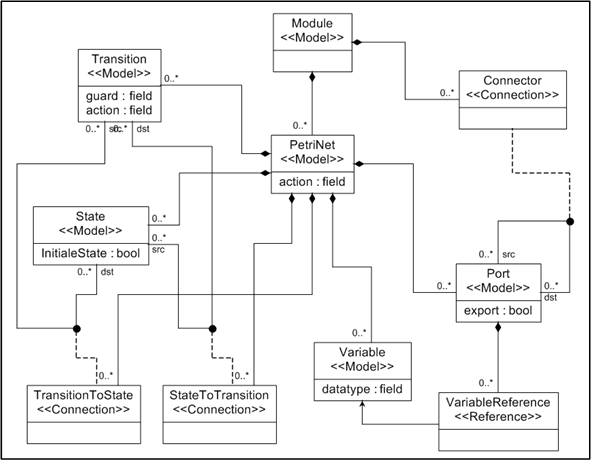
\includegraphics[width=1.00\textwidth]{figures/bip_gme_meta.png}
	\caption{GME Metamodel for restricted BIP Petri net language.}
	\label{fig:bip_gme_meta}
\end{figure}

The BIP GME metamodel (Fig. \ref{fig:bip_gme_meta}) formalizes the structure of a language where each component is specified as a Petri Net.  Petri Net components contain states, transitions, and connections between them. A transition is interpreted as handling a sending or receiving interaction, depending on the connections made to the associated port.  For inbound connections (the destination end of a connector) the transition is triggered by an arriving message.  For outbound connections, the transition sends a message.  

\subsection{Send and Receive translation for interactions}

\begin{figure}[htb]
	\centering
		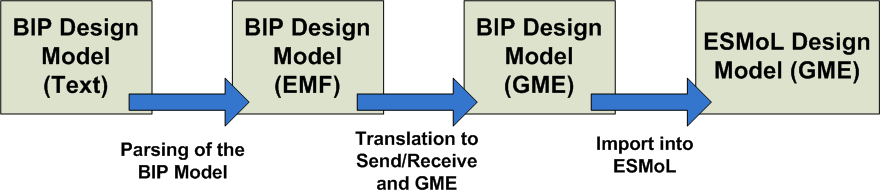
\includegraphics[width=1.00\textwidth]{figures/bip_import.png}
	\caption{Process for importing BIP models into ESMoL.}
	\label{fig:bip_import}
\end{figure}


Todo: Details of the send/receive translation (MJ).

\subsection{Importing into ESMoL}

The ESMoL language is a composite of many sublanguages.  One of those sublanguages is structurally indentical to the BIP metamodel previous described.  The transformation is an isomorphism from a BIP GME model into an ESMoL BIP GME model, but which navigates the structure of the ESMoL model to place the imported data into the right folders.

\subsection{Future work}

\begin{itemize}
\item Figure out how to map rendezvous to locally-deployed components.
\item Figure out how to model and support distributed synchronization.
\end{itemize}
